\section{Resultados e discussão}

Salvo indicação em contrário, os números são média $\pm$ desvio padrão em 10 seeds (Seção~\ref{sec:seeds}); as figuras e os exemplos de erro usam a seed 42. Acurácias e F1 estão em \%; ganhos e superestimativas são relativos.

\subsection{Vazamento por descritores repetidos}\label{sec:vazamento}

Das 27.476 moléculas, 22.699 têm uma tupla de descritores distinta e 4.777 repetem a de outra molécula (o maior grupo tem 12). Nenhum grupo mistura classes. Na divisão aleatória, \gemeas~$\pm$~\sdGemeas\% das moléculas de teste têm uma gêmea de descritores no treino, isto é, outra molécula com exatamente os mesmos cinco valores. O efeito aparece na última coluna da Tabela~\ref{tab:features}: com só os cinco descritores, a divisão aleatória superestima a acurácia em \gapDesc~$\pm$~\sdGapDesc\%, pois a árvore pode decorar as gêmeas. Com as contagens de SMILES o excesso cai para \gapSmiles\% tanto com elas sozinhas quanto com os 17 atributos, porque moléculas com os mesmos descritores têm SMILES diferentes e as contagens não são copiadas junto. A partir daqui, usa-se a divisão agrupada.

\begin{table}[ht]
\centering
\caption{Árvore de decisão no teste, por conjunto de atributos (média $\pm$ desvio em 10 seeds). Cada linha reúne dois cenários da Tabela~\ref{tab:cenarios}. Superestimativa: quanto a acurácia da divisão aleatória excede a da agrupada, em termos relativos.}
\label{tab:features}
\footnotesize
\begin{tabular}{lcccc}
\toprule
Atributos & \shortstack{Acurácia\\aleatória} & \shortstack{Acurácia\\agrupada} & \shortstack{F1 macro\\agrupado} & \shortstack{Superestimativa\\(pontos)} \\
\midrule
Descritores (5) & 0,812 $\pm$ 0,005 & 0,771 $\pm$ 0,008 & 0,770 $\pm$ 0,008 & 4,1 $\pm$ 0,9 \\
SMILES (12) & 0,889 $\pm$ 0,004 & 0,876 $\pm$ 0,006 & 0,873 $\pm$ 0,006 & 1,3 $\pm$ 0,9 \\
Ambos (17) & 0,908 $\pm$ 0,003 & 0,894 $\pm$ 0,004 & 0,893 $\pm$ 0,004 & 1,4 $\pm$ 0,4 \\
\bottomrule
\end{tabular}

\end{table}

\subsection{Efeito dos atributos de SMILES}

Na divisão agrupada, os cinco descritores dão acurácia de \accGrupDesc~$\pm$~\sdGrupDesc\%. As 12 contagens de SMILES sozinhas chegam a \accGrupSmiles~$\pm$~\sdGrupSmiles\%, um ganho relativo de \ganhoSmiles\%. Os 17 atributos juntos chegam a \accGrupAmbos~$\pm$~\sdGrupAmbos\% (F1 macro de \fscoreGrupAmbos\%), um ganho relativo de \ganhoAmbos\% sobre os descritores, muito acima da variação entre seeds. Contar letras de uma cadeia de texto carrega mais informação sobre a molécula, como o número de anéis aromáticos e de halogênios, do que cinco propriedades globais. Na seed 42, a árvore escolhida acerta 89,7\%, dentro da faixa de \faixaMin\% a \faixaMax\% observada nas 10 seeds.

\subsection{Profundidade e poda}

A busca em grade escolheu a entropia como critério e nenhum limite de profundidade nos seis cenários, e só ativou a poda quando os atributos eram apenas os descritores: com cerca de 22 mil linhas de treino, a regra de parada da própria árvore já fica perto do ideal. A Figura~\ref{fig:curvas}a mostra o motivo. A acurácia de treino chega a 100\% na profundidade 25, enquanto a de validação estaciona em torno de 87\% a partir da profundidade 16. A poda por custo-complexidade (Figura~\ref{fig:curvas}b) reduz a árvore de 2.054 para 899 folhas com $\alpha = 10^{-4}$ sem perder acurácia de validação (87,0\% para 87,2\%); acima de $10^{-3}$ a poda passa a custar acurácia, e com $\alpha = 10^{-2}$ sobram 8 folhas e 66,5\%.

\begin{figure}[ht]
\centering
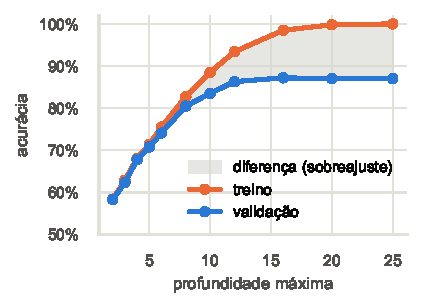
\includegraphics[width=.49\textwidth]{figures/depth_curve.pdf}\hfill
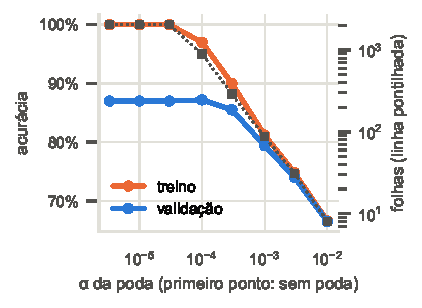
\includegraphics[width=.49\textwidth]{figures/pruning_curve.pdf}
\caption{Acurácia de treino e de validação (seed 42, divisão agrupada, 17 atributos). (a) Por profundidade máxima. (b) Por $\alpha$ da poda, com o número de folhas na escala da direita (linha pontilhada); o primeiro ponto é $\alpha=0$.}
\label{fig:curvas}
\end{figure}

\subsection{O que a árvore aprendeu}

A árvore escolhida tem 1.854 folhas e 24 níveis, grande demais para ser desenhada. As primeiras camadas, porém, são legíveis. A raiz divide por TPSA (limiar de 67,9) e o ramo de TPSA baixa tem 69\% de DRD2, como a análise exploratória antecipava. Em seguida vêm o número de átomos aromáticos, um atributo do SMILES, e depois HBD, número de anéis, comprimento do SMILES e número de halogênios. Descritores e contagens se misturam já no topo. A Figura~\ref{fig:import} confirma o quadro: TPSA e o número de átomos aromáticos lideram nas duas medidas de importância, seguidos por HBD e por um bloco de contagens (átomos de N, halogênios, estereoquímica, anéis) acima de LogP e HBA. A importância por permutação, medida no teste, dá mais peso às contagens do que a de impureza.

\begin{figure}[ht]
\centering
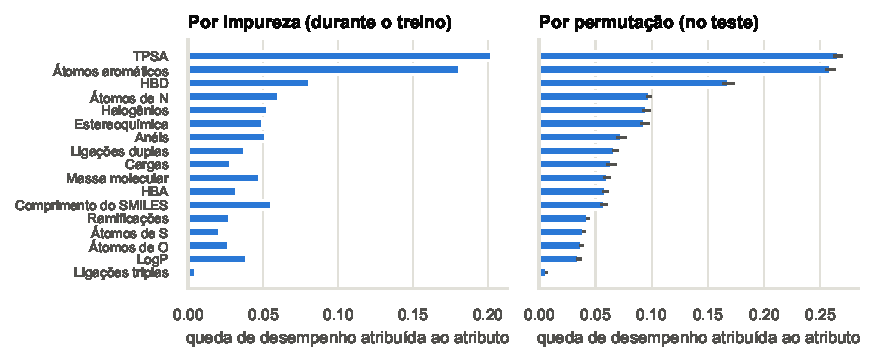
\includegraphics[width=\textwidth]{figures/feature_importances.pdf}
\caption{Importância dos atributos da árvore escolhida (seed 42). À esquerda, a redução de impureza acumulada nos nós que usam o atributo, durante o treino. À direita, a queda de acurácia no teste quando os valores do atributo são embaralhados (permutação).}
\label{fig:import}
\end{figure}

\subsection{Erros e limites da árvore}

Entre as classes, BACE1 e DRD2 são as mais fáceis (F1 de \fscoreBACEone\% e \fscoreDRDtwo\%), seguidas de EGFR (\fscoreEGFR\%) e HDAC1 (\fscoreHDACone\%), a mais difícil. Na seed 42, o par HDAC1 $\leftrightarrow$ EGFR, nos dois sentidos, soma 28,7\% dos 568 erros (Figura~\ref{fig:erros}a), e 7,9\% das moléculas de HDAC1 viram EGFR. Os erros não ocupam uma região do espaço de atributos: nenhum dos 17 atributos desloca a mediana entre acertos e erros em mais de meio intervalo interquartil. Entre seis exemplos de HDAC1 lidos como EGFR, dois contêm a mesma subestrutura, o grupo de átomos C(=O)NO. A árvore não a distingue: contagens de caracteres dizem quantos oxigênios e nitrogênios existem, mas não como estão ligados.

A árvore também não sabe quando erra. Sem poda, toda folha é pura, então a probabilidade de classe estimada pela árvore é 100\% nas 5.496 previsões de teste, embora 10,3\% estejam erradas. A curva de aprendizado (Figura~\ref{fig:erros}b) mostra a outra limitação: o treino fica em 100\% e a validação sobe de 61,5\% (879 linhas) para 87,0\% (17.584) sem se achatar, de modo que mais moléculas provavelmente renderiam mais acurácia.

\begin{figure}[ht]
\centering
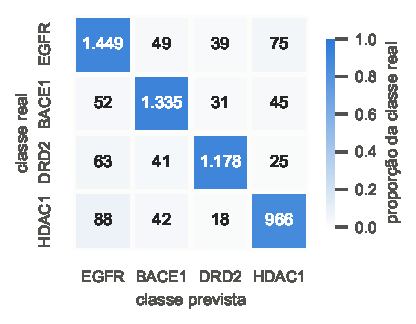
\includegraphics[width=.44\textwidth]{figures/confusion_matrix.pdf}\hfill
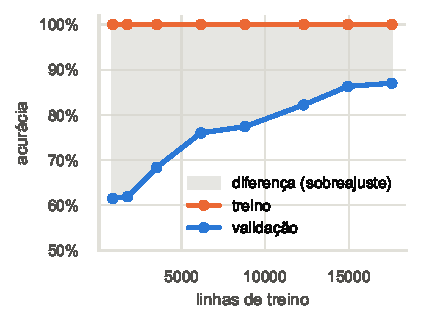
\includegraphics[width=.52\textwidth]{figures/learning_curve.pdf}
\caption{Seed 42, divisão agrupada, 17 atributos. (a) Matriz de confusão no teste: cor pela proporção da classe real, número em contagem. (b) Curva de aprendizado: acurácia por tamanho do conjunto de treino.}
\label{fig:erros}
\end{figure}

\subsection{Comparação com modelos de referência}

A Tabela~\ref{tab:referencia} situa a árvore entre um piso e um teto. Responder sempre EGFR, a classe majoritária, dá \accMaj\% de acurácia, que é a proporção de EGFR na base. A Random Forest~\cite{breiman:01} chega a \accRF~$\pm$~\sdRF\% e o \emph{gradient boosting} a \accHGB~$\pm$~\sdHGB\%, enquanto a árvore única acerta \accArvore~$\pm$~\sdArvore\%: a Random Forest supera a árvore em \ganhoRF\% (relativo). Esse ganho é o preço da interpretabilidade: a árvore responde por que uma molécula foi classificada como DRD2 com um caminho de perguntas sobre TPSA e contagens, enquanto os conjuntos não têm regras legíveis.

\begin{table}[ht]
\centering
\caption{Árvore e modelos de referência na divisão agrupada, com os 17 atributos (média $\pm$ desvio em 10 seeds).}
\label{tab:referencia}
\footnotesize
\begin{tabular}{lcc}
\toprule
Modelo & Acurácia & F1 macro \\
\midrule
Classe majoritária & 0,293 $\pm$ 0,000 & 0,113 $\pm$ 0,000 \\
Árvore de decisão & 0,894 $\pm$ 0,004 & 0,893 $\pm$ 0,004 \\
Random Forest (300 árvores) & 0,952 $\pm$ 0,003 & 0,951 $\pm$ 0,003 \\
HistGradientBoosting & 0,948 $\pm$ 0,003 & 0,947 $\pm$ 0,003 \\
\bottomrule
\end{tabular}

\end{table}
